\section{Theory}

% CUE 5 | 0:50 | 이토 보조정리와 변동성 항력의 수리적 도출
\begin{frame}{이토 보조정리(Ito's Lemma)와 변동성 항력의 엄밀한 도출}
\textbf{연속시간 기하 브라운 운동 (GBM)} 하에서 자산 가격 $S_t$의 확률과정:
\begin{equation*}
  dS_t = \mu S_t dt + \sigma S_t dW_t \quad (W_t: \text{표준 위너 과정})
\end{equation*}

여기에 로그 효용/연속 복리 성장 함수 $f(S_t) = \ln S_t$를 적용하고 2계 테일러 전개 전개식에 이토 공식 $(dW_t)^2 = dt$를 대입:
\begin{equation*}
  d\ln S_t = \frac{\partial f}{\partial S_t} dS_t + \frac{1}{2} \frac{\partial^2 f}{\partial S_t^2} (dS_t)^2 = \frac{1}{S_t}(\mu S_t dt + \sigma S_t dW_t) + \frac{1}{2}\left(-\frac{1}{S_t^2}\right)(\sigma^2 S_t^2 dt)
\end{equation*}

\vspace{1mm}
\begin{block}{단일 자산 연속 복리 성장률 정리}
  \centering
  \large
  $d\ln S_t = \underbrace{\left( \mu - \frac{1}{2}\sigma^2 \right)}_{g \text{ (연속 복리 기하성장률)}} dt + \sigma dW_t \implies \mathbf{g = \mu - \frac{1}{2}\sigma^2}$
\end{block}

\vspace{1mm}
\begin{itemize}
  \small
  \item \textbf{변동성 항력 (Volatility Drag)}: $\boldsymbol{\Delta \equiv \mu - g = \frac{1}{2}\sigma^2}$
  \item 자산의 기대수익률($\mu$)이 동일하더라도, 변동성($\sigma$)이 2배가 되면 자본 잠식 손실은 \textbf{4배($2^2$)}로 급증함.
\end{itemize}
\end{frame}

% CUE 6 | 0:45 | 에르고딕성 붕괴와 레버리지 L^2 급증 메커니즘
\begin{frame}{에르고딕성 파괴(Peters, 2019)와 레버리지 $L^2$ 급증 메커니즘}
\begin{columns}[T]
  \begin{column}{0.48\textwidth}
    \textbf{에르고딕성(Ergodicity)의 파괴}
    \begin{itemize}
      \setlength{\itemsep}{4pt}
      \small
      \item \textbf{앙상블 평균 ($\mu$, 공간적 기대치)}:
      무한한 평행우주 투자자들의 평균 수익률.
      \item \textbf{시간 평균 ($g$, 단일 궤적 복리)}:
      단 하나의 시간 축을 살아가는 실제 투자자의 실질 부.
      \item 금융 시장은 곱셈적 확률 과정이므로 \textbf{앙상블 평균 $\neq$ 시간 평균} (Peters, 2019 \textit{Nature Physics}).
    \end{itemize}
    
    \vspace{2mm}
    \textbf{레버리지 자산의 $L^2$ 항력 폭증}
    \begin{itemize}
      \setlength{\itemsep}{4pt}
      \small
      \item $L$배 레버리지 ETF의 복리 성장률:
      $g_L = L\mu - \frac{1}{2}(L\sigma)^2 = L\mu - \mathbf{L^2}\left(\frac{1}{2}\sigma^2\right)$
      \item 변동성 항력이 \textbf{$L^2$배로 가속 침식} (2x는 4배, 3x는 9배).
    \end{itemize}
  \end{column}
  
  \begin{column}{0.50\textwidth}
    \centering
    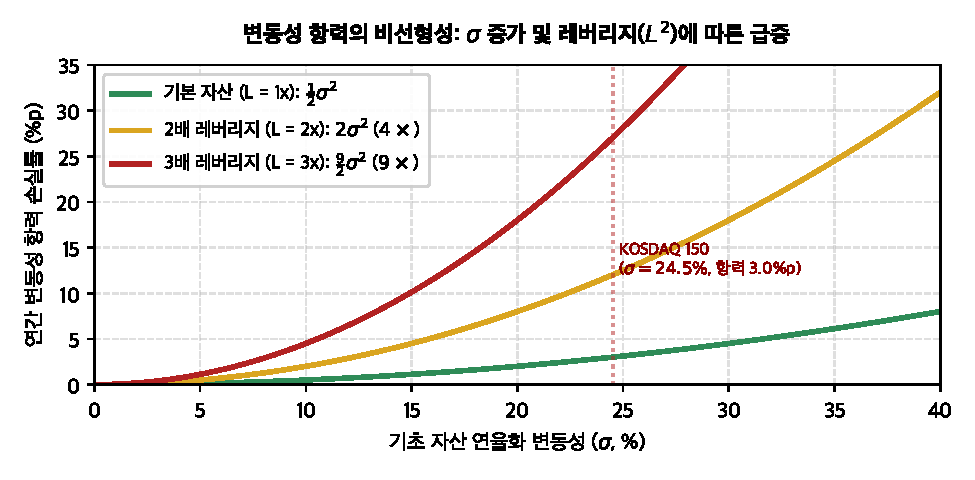
\includegraphics[width=\linewidth]{MyFigure/drag_vs_sigma.pdf}
    \vspace{-2mm}
    \begin{exampleblock}{KOSDAQ 150 항력 검증: 제출본 vs 실데이터}
      \scriptsize
      \begin{tabular}{@{}lccc@{}}
        & $\sigma$ & 실측 항력 & $\frac{1}{2}\sigma^2$ \\
        \textbf{제출본} <표 1-A> & 24.53\% & 3.00\%p & 3.01\%p \\
        \textbf{사전등록 실데이터} & 30.47\% & 4.63\%p & 4.64\%p \\
      \end{tabular}\\
      실데이터 7개 자산 최대 $|\Delta| = 0.014\%p$ (2015.01$\sim$2026.08)
    \end{exampleblock}
  \end{column}
\end{columns}
\end{frame}

% CUE 7 | 0:45 | 켈리 목적함수와 이토 보정 볼록 최적화
\begin{frame}{다변량 복리 최적화: 켈리 기준($\lambda=1$)과 이토 보정 Convex QP}
\textbf{다변량 포트폴리오의 연속 복리 성장률 도출} (가중치 벡터 $\mathbf{w}$):
\begin{equation*}
  g_p(\mathbf{w}) = \mathbf{w}^\top \boldsymbol{\mu} - \frac{1}{2} \mathbf{w}^\top \boldsymbol{\Sigma} \mathbf{w}
\end{equation*}

\begin{block}{전통 MVO 목적함수와의 본질적 차이}
  \small
  \begin{itemize}
    \item \textbf{마코위츠 MVO}: $\max_{\mathbf{w}} \mathbf{w}^\top \boldsymbol{\mu} - \frac{\lambda}{2} \mathbf{w}^\top \boldsymbol{\Sigma} \mathbf{w}$ ($\lambda$는 주관적 위험회피계수로 임의 설정)
    \item \textbf{제안 모델 (Itô-Kelly)}: 이토 보조정리에 의해 장기 복리 성장률 극대화 시 위험 페널티 계수는 \textbf{수학적으로 반드시 $\boldsymbol{\lambda=1}$로 고정됨}!
  \end{itemize}
\end{block}

\vspace{1mm}
\textbf{Rockafellar-Uryasev (2000) 95\% CVaR 선형화 상한 제약의 결합}:
\begin{equation*}
  \max_{\mathbf{w}, \alpha, \mathbf{u}} \left[ \mathbf{w}^\top \hat{\boldsymbol{\mu}}_t - \frac{1}{2} \mathbf{w}^\top \hat{\boldsymbol{\Sigma}}_t \mathbf{w} \right] \quad
  \text{s.t.} \quad 
  \begin{cases}
    \alpha + \frac{1}{J(1-\gamma)} \sum_{j=1}^J u_j \le \text{CVaR}_{\text{target}} \\
    u_j \ge -\mathbf{w}^\top \mathbf{r}_j - \alpha, \quad u_j \ge 0 \\
    \mathbf{1}^\top \mathbf{w} = 1, \quad 0 \le w_i \le 0.40 \quad (\text{공매도 금지})
  \end{cases}
\end{equation*}

\vspace{1mm}
$\implies$ 엄격한 오목성(Strict Concavity)을 지닌 \textbf{볼록 2차 계획법(Convex QP)}으로 전역 최적해 유일 수렴 보장.
\end{frame}
